\section{Analyse et Conception du Project}
\subsection{Analyse fonctionnelle}
\begin{frame}{Analyse du besoin}
    \begin{figure}[H]
        \centering
        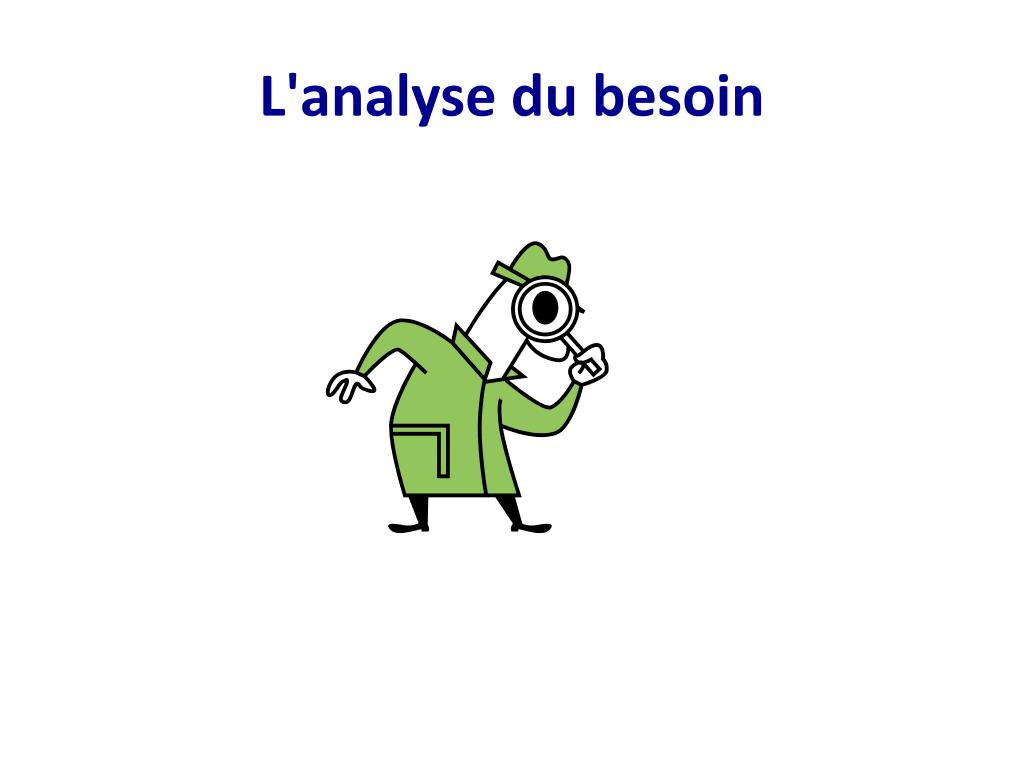
\includegraphics[height=5cm]{assets/images/analyse-besoin.jpg}
    \end{figure}

\end{frame}

\begin{frame}{Digramme cas d'utilisation}
    \begin{figure}[H]
        \centering
        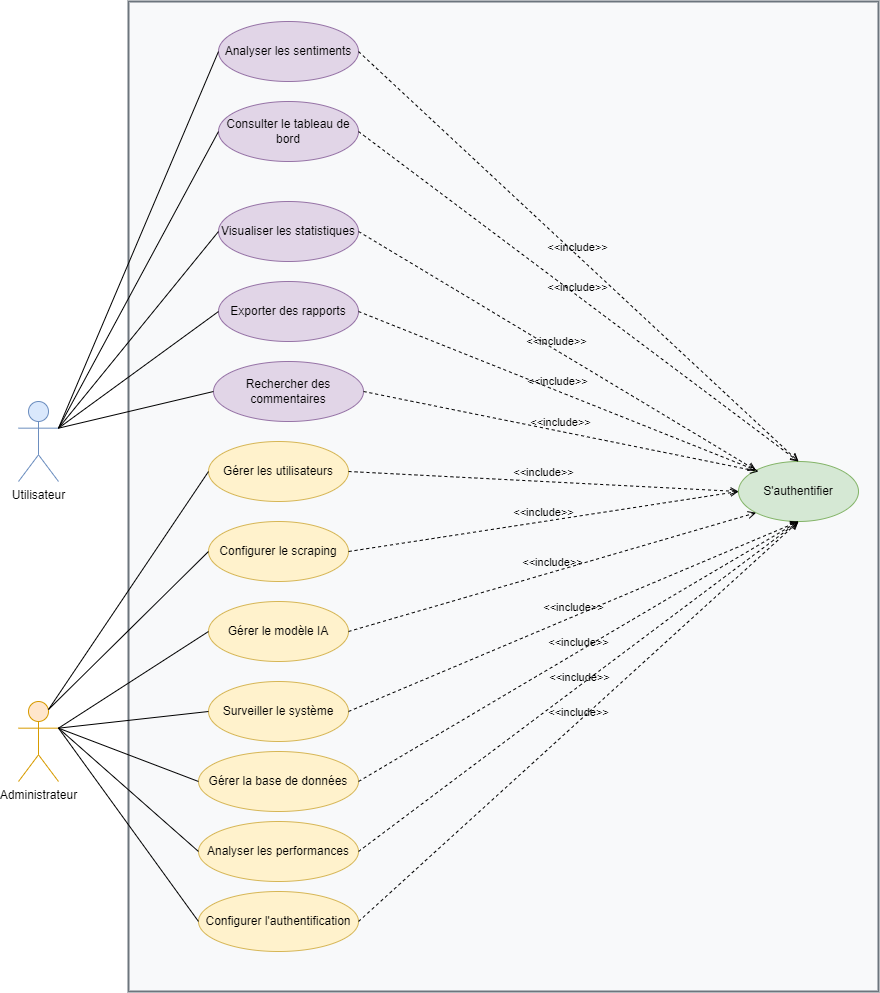
\includegraphics[height=5cm]{assets/images/usecase.png}
    \end{figure}
\end{frame}
\begin{frame}{Digramme cas d'utilisation - Utilisateur}
    \begin{figure}[H]
        \centering
        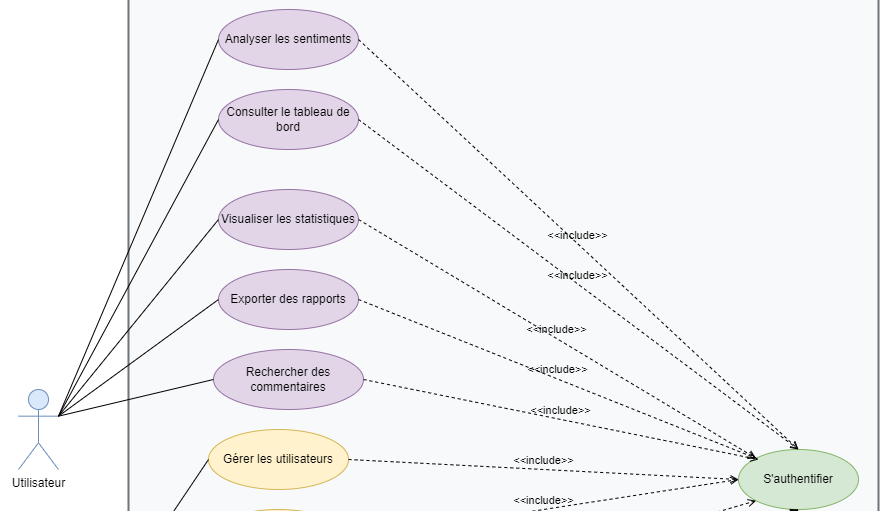
\includegraphics[height=5cm]{assets/images/usecase-user.png}
    \end{figure}
\end{frame}

\begin{frame}{Digramme cas d'utilisation - Admin}
    \begin{figure}[H]
        \centering
        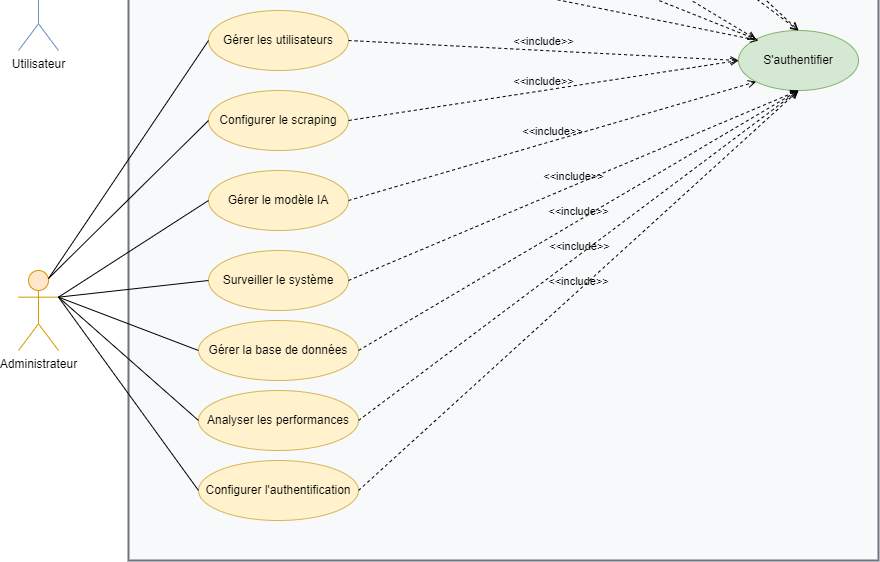
\includegraphics[height=5cm]{assets/images/usecase-admin.png}
    \end{figure}
\end{frame}

\subsection{Analyse technique}

\begin{frame}{Architecture microservice}
    \begin{figure}[H]
        \centering
        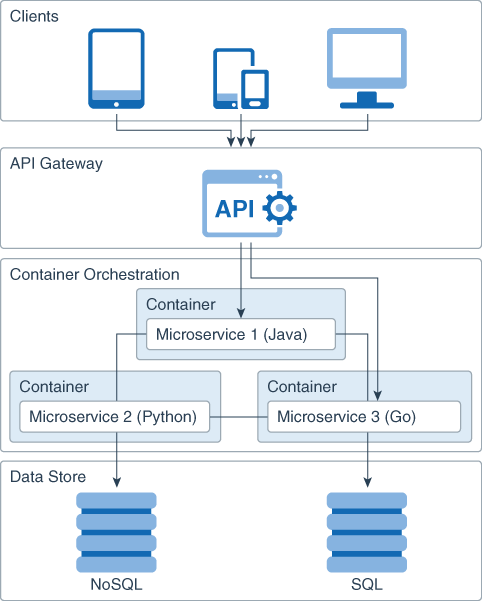
\includegraphics[height=6cm]{assets/images/microservice_arch.png}
    \end{figure}
\end{frame}




\subsection{Methodology}
\begin{frame}{Methodology}

    \begin{figure}[H]
        \centering
        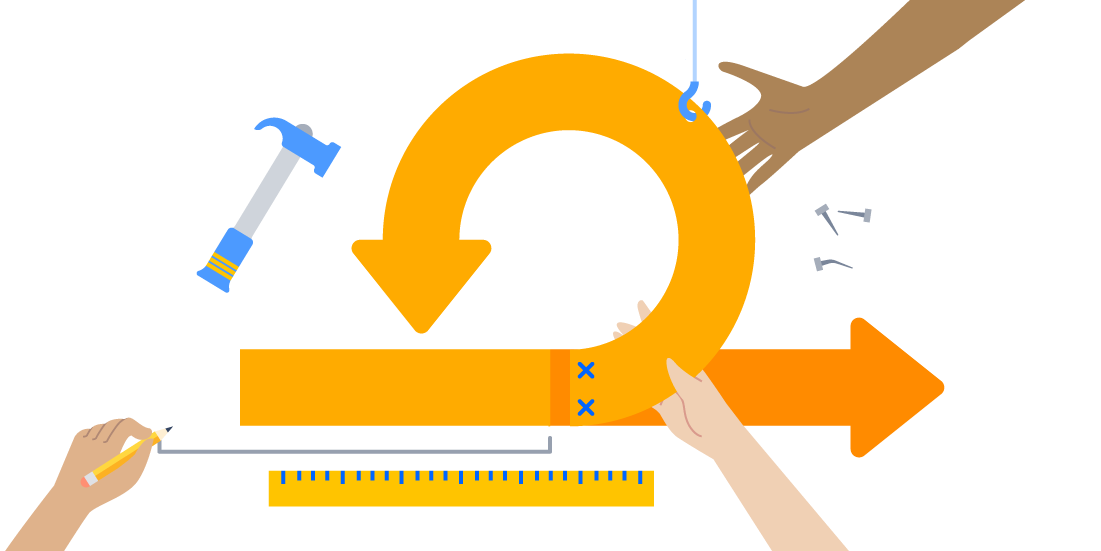
\includegraphics[height=4cm]{assets/images/scrum.png}
    \end{figure}

    Afin de gérer au mieux ce projet, nous avons opté pour la méthode SCRUM et divisé les différents modules en sprints.
\end{frame}


\subsection{Planification}
\begin{frame}{Planification}

    \begin{figure}[H]
        \centering
        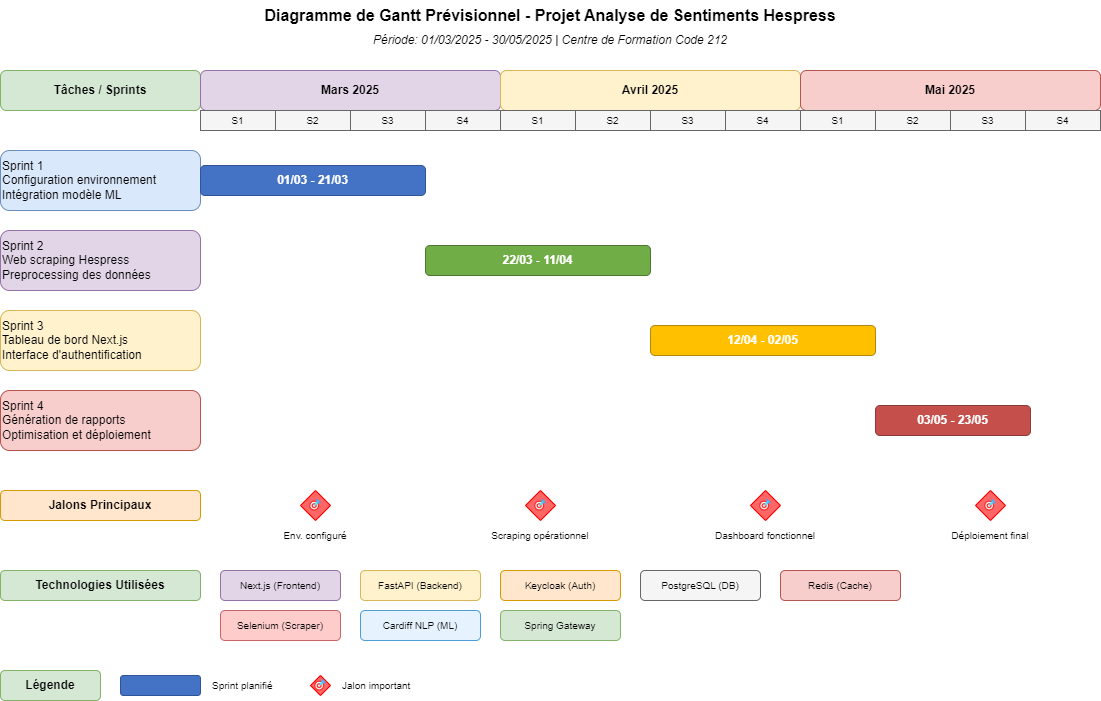
\includegraphics[scale=0.3]{assets/images/gantt-previsionnel.png}
    \end{figure}
\end{frame}





